\chapter{Transient Noise Detection}\label{ch:TransientNoiseDetection}

\ifpdf
    \graphicspath{{Chapter5_TransNoiseDet/Chapter5Figs/PNG/}{Chapter5_TransNoiseDet/Chapter5Figs/PDF/}{Chapter5_TransNoiseDet/Chapter5Figs/}{Chapter5_TransNoiseDet/Chapter5Figs/NoiseBurstModel/}{Chapter5_TransNoiseDet/Chapter5Figs/ARFilterMethod/}}
\else
    \graphicspath{{Chapter5_TransNoiseDet/Chapter5Figs/EPS/}{Chapter5_TransNoiseDet/Chapter5Figs/}}
\fi

The rapid increase in availability of high speed internet connections has made personal computers a popular basis for teleconferencing applications. While embedded microphones, loudspeakers and webcams in laptop computers have made setting up conference calls very easy, it has also brought with it some specific noise difficulties such as feedback, fan noise and button clicking noise. The latter has been a particularly persistent problem and is generally due to the mechanical pulses caused by keystrokes. Particularly on laptop computers this can be a significant nuisance due to the mechanical connection between microphone, within in the laptop case, and the keyboard, and the distinct tactile interface points throughout the key travel. The noise impulses produced can vary greatly with factors such as keystroke speed and length, microphone placement and response, laptop frame or base, keyboard or trackpad type and even surface on which the computer is placed.

The focus of our noise reduction efforts will purely be on the perspective of the receiving end since this is the only noise accessible to us through signal processing, but also since the acoustical feedback from keyboards is often an important cue for the typist, whereas to the receiver it will uncorrelated with any actions.

As noted in the literature review, chapter~\ref{sec:LitRev_Detection}, a range of approaches has been taken to detect impulsive noise in speech and audio. In general the approaches taken can be divided into two categories. The ones that focus on corruptions caused by mechanical defects in the medium or errors in the communication channel and corruptions caused by acoustically additive noise such as transient noise events like hand claps, keyboard strokes and mouse button clicks. Although, as noted in chapter~\ref{sec:LitRev_Detection}, there is an overlap between the applications and the methods used, the focus of this chapter will be the detection of acoustically additive transient noise events, specifically keyboard stroke noise, which are characterised by their length, sequence of multiple pulses and in certain cases significant tonal components.

Chapters~\ref{ch:TransientNoiseDetection} and \ref{ch:TransientNoiseRestoration} can be seen as two stages of the same application. Localised removal of transient noise for realtime applications. In this chapter the focus will be on the initial stage of this system, the detection. This chapter will start with an investigation into the noise pulses in question and the specific parameters related to these pulses. A range of detection algorithms will then be proposed in section~\ref{sec:WPdetection} after which the methods used to evaluate the algorithms will be introduced. The chapter will finish with the presentation and discussion of results and conclusions from the work undertaken.

\section{A look at the data}\label{sec:WPdata}
Figure~\ref{fig:TypingSPLKeyboards} shows a plot of the A-weighted sound pressure level (SPL) of 4 different keyboard pulses aligned\cite{Hauswirth2013}. This data was recorded with an artificial binaural head measurement system in an anechoic environment and as such only serves to outline audible real world acoustic scenario of keystroke pulses. The data clearly shows some key features of keyboard noise.
\begin{enumerate}
\item The length of keyboard strokes can be upwards of 350 ms.
\item In all tested cases the pulses consist of at least 2 clearly defined pulses.
\item The majority of the energy lies in the initial pulse.
\end{enumerate}

The number 2 pulse seen for every device in Figure~\ref{fig:TypingSPLKeyboards} shows what will be referred to as the \emph{lift} pulse from this point onwards. This pulse is related to the physical key or switch returning to its original unpressed position. The relationship between the two pulses are not consistent across different devices and Laptop 1 specifically was said to have a ``hard return stop'' while Laptop 3 has a ``soft return stop'' with a SPL level difference of almost nothing and 18 dB(A) SPL respectively.

\begin{figure}[!] %TypingSPLKeyboards
\centering
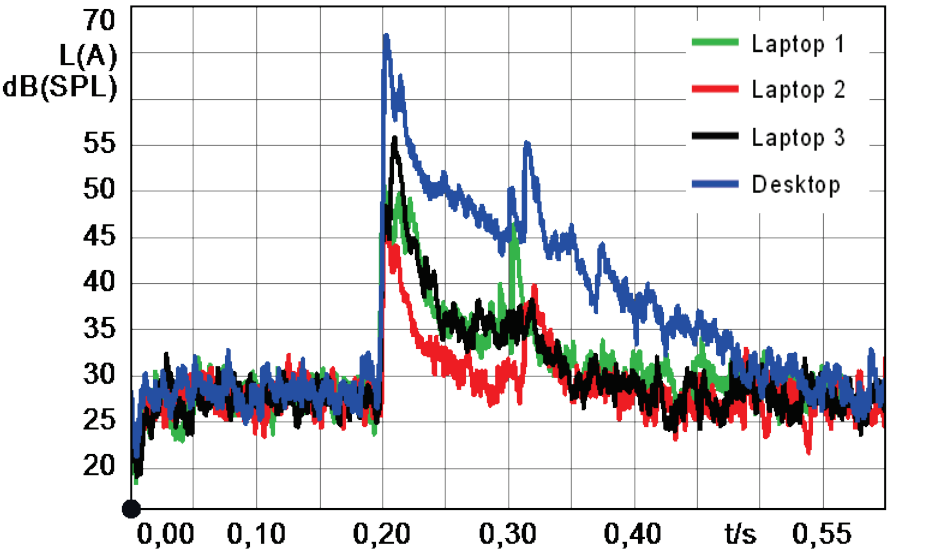
\includegraphics[width=100mm]{TypingSPLKeyboards.png}
\caption{SPL analysis of keyboard noise (time weighting: 2ms). Plot reproduced from \cite{Hauswirth2013}.}\label{fig:TypingSPLKeyboards}
\end{figure}

Figure~\ref{fig:TypingLoudnessKeyboards} shows the loudness of keyboard pulses versus time. Loudness is a representation of a human's perception of sound volume and is represented on a linear scale so that twice the loudness represents a listener perceiving the sound twice as loud. The figure shows that the desktop keyboard is perceived as being over twice as loud as a laptop keyboard. Desktop keyboards are traditionally optimised for typing comfort and tactile feedback while not having to consider the spacial constraints of laptop computers. In addition some keyboards are specifically designed to give the user audible feedback\cite{Hauswirth2013}.

\begin{figure}[!] %TypingLoudnessKeyboards
\centering
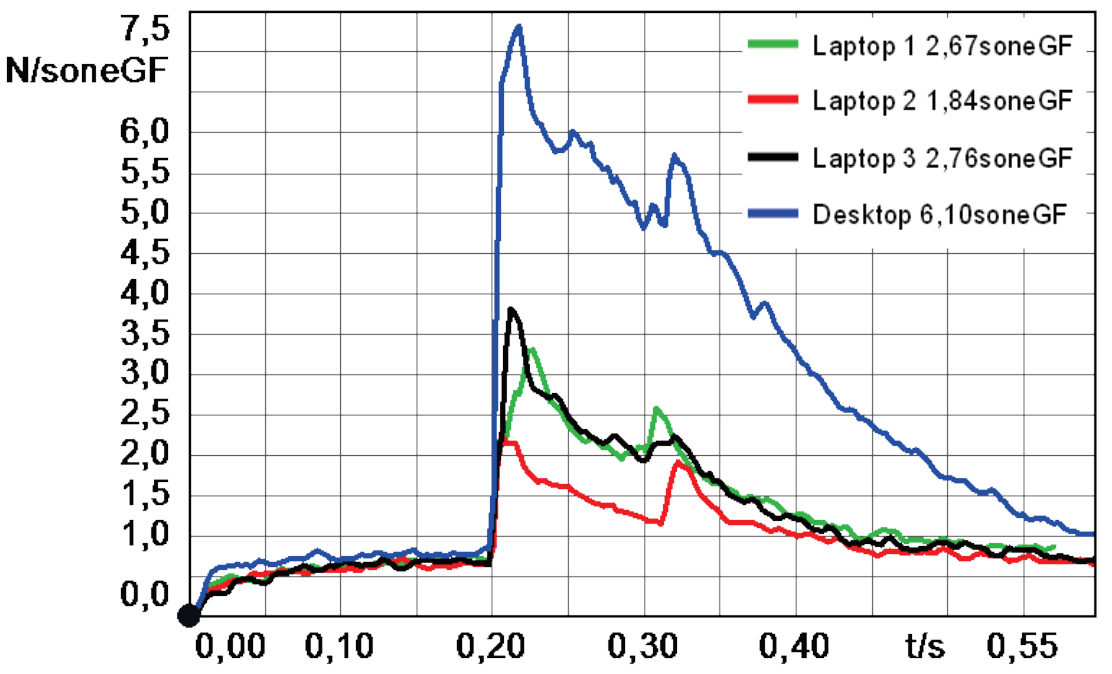
\includegraphics[width=100mm]{TypingLoudnessKeyboards.png}
\caption{Loudness analysis of keyboard noise. Plot reproduced from \cite{Hauswirth2013}.}\label{fig:TypingLoudnessKeyboards}
\end{figure}

In addition to the loudness, Figure~\ref{fig:TypingLoudnessKeyboards} also shows the 5\% percentile value as a single number in the diagram legend. This value indicated the value which the signal exceeds during 5\% of the examined time interval\cite{Hauswirth2013}. This number also reflects the fact that the desktop keyboards in general are perceived much more loudly than laptop keyboards so while laptop keyboards are of interest due to their mechanical connection and physical proximity to the microphone, desktop keyboards is clearly also a potential source of nuisance in telecommunication applications.

\subsection{Spectral investigation of audio signals}
Figure~\ref{fig:spectrogramMarkedTapsBrownFox} shows a spectrogram of a short sequence of speech with typing strokes embedded in it. The figure overlays show the approximate positions of the strokes in the spectrogram. It can be observed that the typing strokes have a fairly flat frequency response compered to the the voiced parts of the audio sequence.

\begin{figure}[!] %spectrogramMarkedTapsBrownFox
\centering
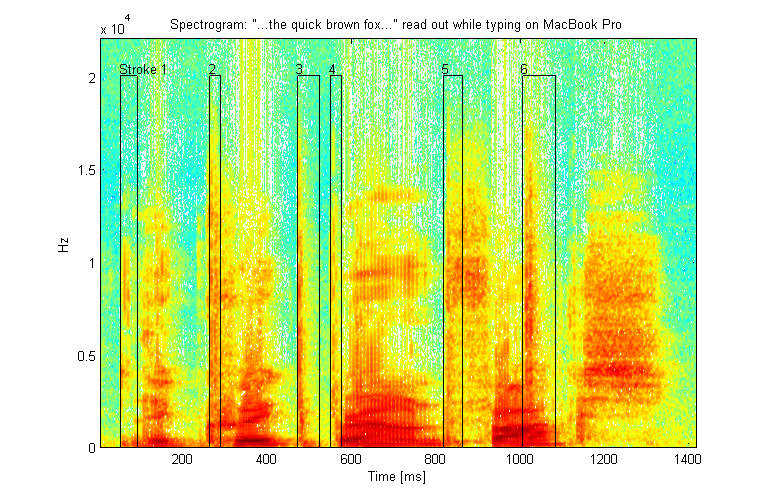
\includegraphics[width=150mm]{spectrogramMarkedTapsBrownFox.png}
\caption{Spectrogram analysis of mixed typing strokes and speech. Overlay shows positions of typing strokes.}\label{fig:spectrogramMarkedTapsBrownFox}
\end{figure}

Figure~\ref{fig:waveletspectrumAno} shows the wavelet spectrum of a sequence of keystrokes with speech interference. The figure overlays show the approximate positions of the strokes in the wavelet spectrum.
\begin{figure}[!] %waveletspectrumAno
\centering
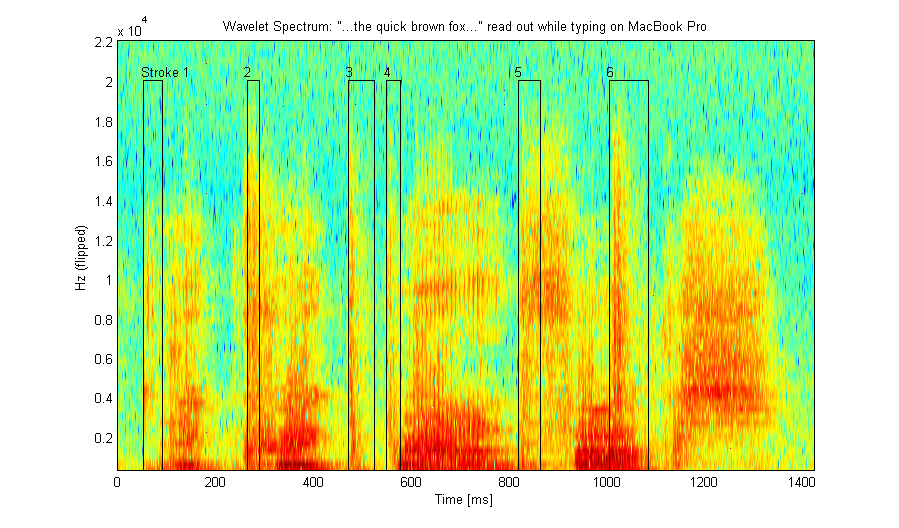
\includegraphics[width=150mm]{waveletspectrumAno.png}
\caption{Top: Waveform of typing sequence. Bottom: Wavelet spectrum of same typing sequence.}\label{fig:waveletspectrumAno}
\end{figure}

\subsection{Keystroke sequence investigation}
A single keystroke, during rapid typing and not at the end of a typing sequence, is generally made up of 3 primary sections.
\begin{enumerate}
  \item A primary \textbf{Stroke} keystroke (15 - 40 ms),
  \item a \textbf{Break} while key is depressed (50 - 500 ms) and
  \item a \textbf{Lift} pulse (15 - 40 ms).
\end{enumerate}
The duration of the break region will typically be determined by the typing speed of the user while the Stroke and the Lift region are primarily constant and will vary more with factors such as stroking force and the vibrational characteristics of the keyboard and the laptop casing.

Figure~\ref{fig:KeyboardStrokeSlow} shows a waveform of a single typing stroke. The waveform clearly shows the two distinct pulses of sudden erratic excitation followed by a slowly decaying low frequency sinusoid.

\begin{figure}[!] %KeyboardStrokeSlow
\centering
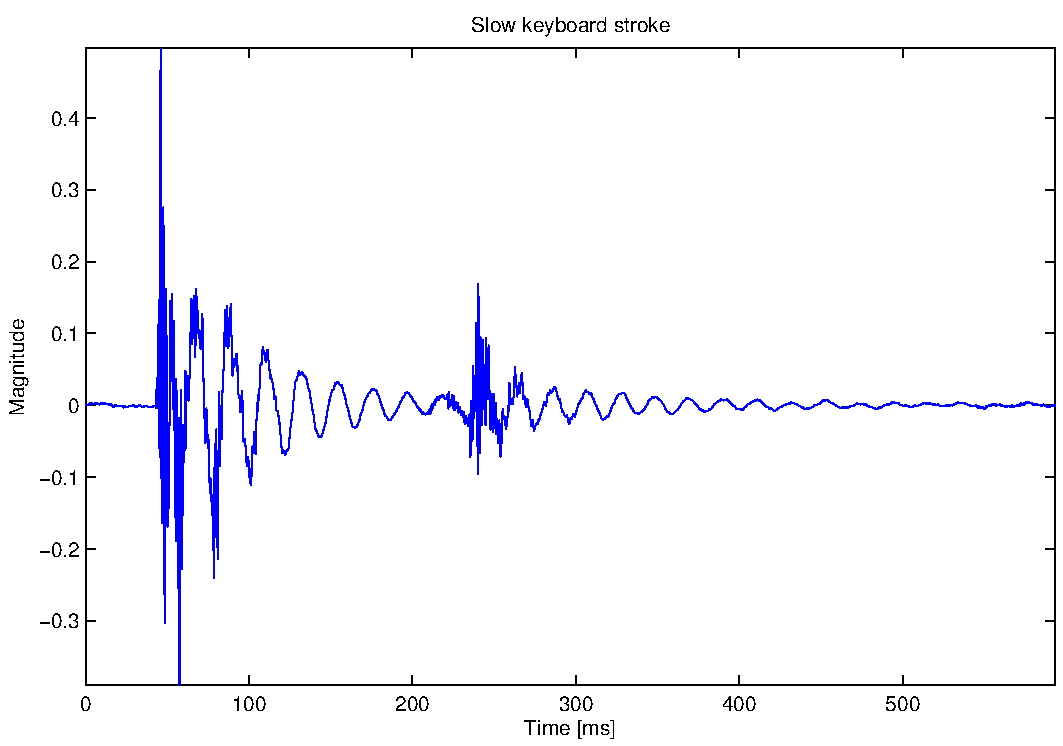
\includegraphics[width=120mm]{KeyboardStrokeSlow.pdf}
\caption{Single slow keyboard stroke.}\label{fig:KeyboardStrokeSlow}
\end{figure}

Figure~\ref{fig:Keyboard2StrokesFast} shows a sequence of two keystrokes in rapid succession. The keystroke regions mentioned above are clearly annotated with their temporal extent also noted.

\begin{figure}[!] %Keyboard2StrokesFast
\centering
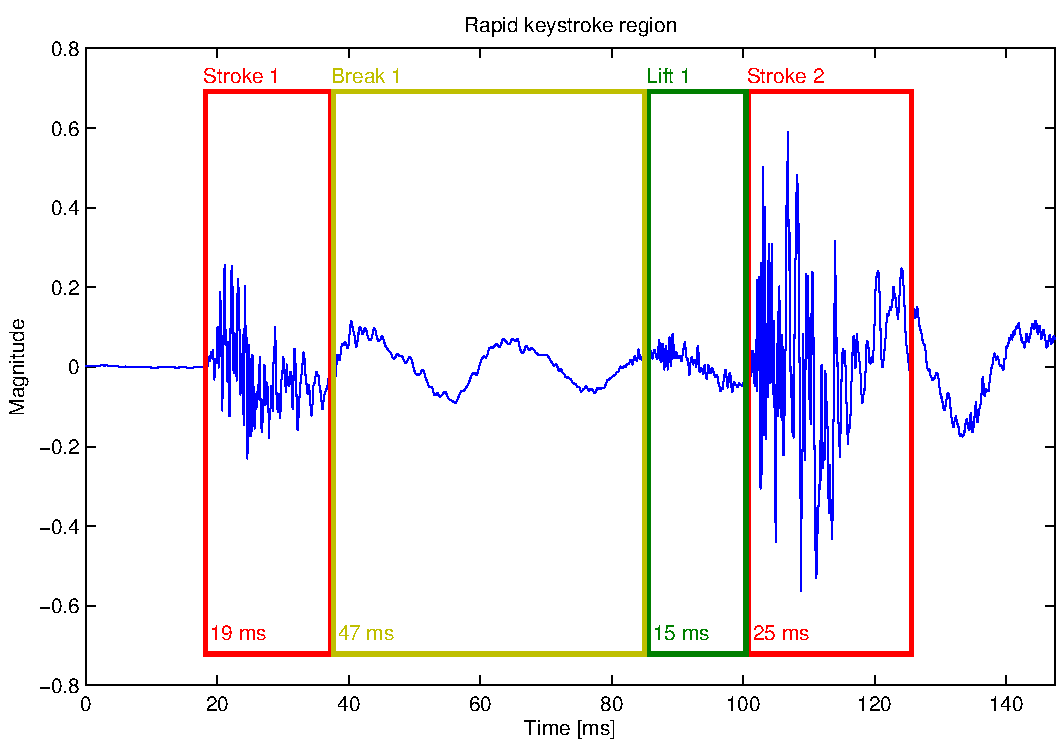
\includegraphics[width=120mm]{Keyboard2StrokesFast.pdf}
\caption{Two annotated keyboard strokes in rapid succession.}\label{fig:Keyboard2StrokesFast}
\end{figure}

Figure~\ref{fig:Keyboard4StrokesFast} shows an example of a short rapid 4 keystroke sequence.

\begin{figure}[!] %Keyboard4StrokesFast
\centering
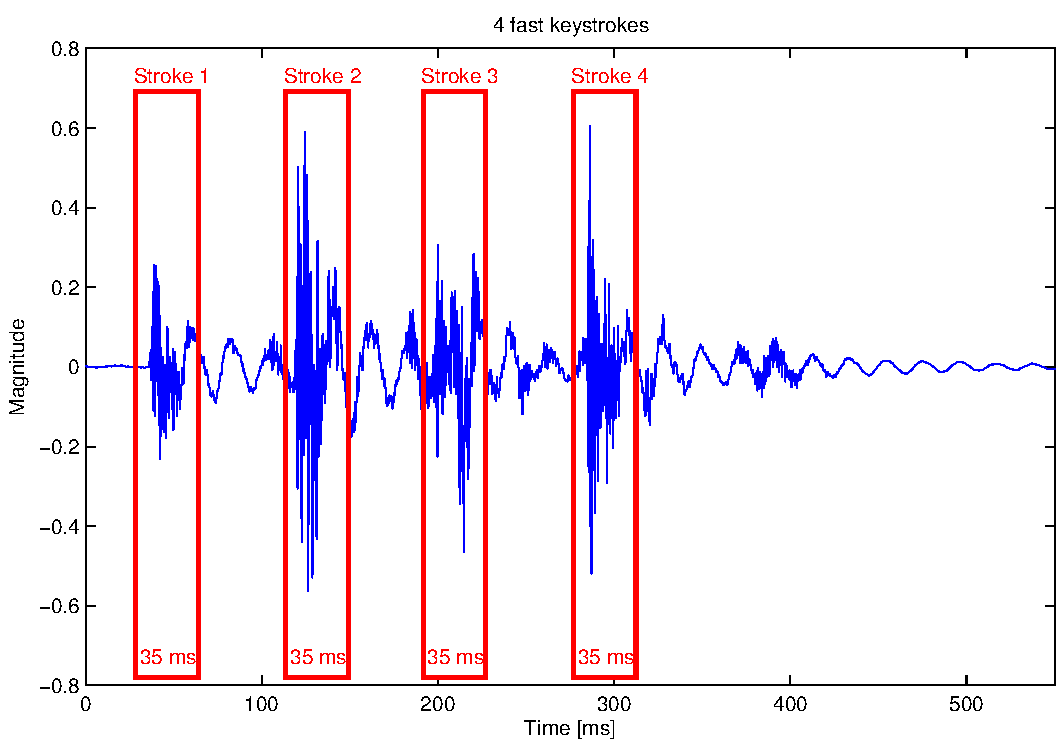
\includegraphics[width=120mm]{Keyboard4StrokesFast.pdf}
\caption{Four annotated keyboard strokes in rapid succession.}\label{fig:Keyboard4StrokesFast}
\end{figure}

\section{Detection algorithms}\label{sec:WPdetection}
The basic detection algorithm is comprised of two stages. First a separation stage aims to separate the transient noise pulses by separating out tonal atoms assumed to be speech components and secondly a detection stage which attempts to detect transient noise events through the wavelet bases. For the detection stage 2 different approaches has been explored.

\subsection{Separation pre processing}\label{sec:WPseparation}
%good amplitude results in \cite{Vaseghi1990}
The purpose of the separation stage is twofold. Firstly the removal of tonal atoms, and thereby speech, should aid in the detection algorithms ability to distinguish between speech signals and transient noise. Secondly, the tonal atoms provide a good first approximation for a restoration, equally the residual signal, used for detection, should ideally be a sparse signal containing mainly the transient noise events. Methods utilizing similar approaches in the literature clearly documents its advantages\cite{Godsill1998book} (see section~\ref{sec:LitRevAR} for full review). Visual examples produced in section~\ref{sec:WPseparation} and audible examples provided \sound{Separation examples} also speaks to the power of the separation pre processing stage.
Future restoration efforts should therefore mainly be focused on the residual signal and, in general, the scope of the detrimental effects of restoration should be limited.

The incoming audio signal can be expressed as the linear combination of a voiced signal and a sparse signal containing the transient noise events:
\begin{equation}\label{eq:modelgeneral}
    x(n) = \sum_i c_i \Phi_i(n) + \sum_{j} w_{j}(n) \Psi_{j}(n),
\end{equation}
where $c_i$ are the coefficients for the voiced parts of the signal and $\Phi$ is the standard short-time Fourier basis. $w_{j}(n)$ are the coefficients of the residual where $j$ is an integer relating to some translation and dilation of some Wavelet basis function $\Psi$. Here we are utilising an overcomplete dictionary of atoms to represent the audio: a dictionary of `tonal' atoms and a dictionary of `transient' atoms that are aimed at capturing voiced speech and transient noise, respectively. Multiple dictionaries have been employed in Bayesian probabilistic methodologies for noise reduction purposes in \cite{Fevotte2006}\cite{Fevotte2008} (see also references therein for other approaches with multiple dictionaries). \todo{Maybe remove this: }Here we focus on development of a fast algorithm using the principles of the above model in order to first extract the tonal (voiced) components in order to process the noise components directly in the wavelet domain. Other tonal dictionaries such as Gabor functions and other transient dictionaries such as standard discrete or continuous wavelet transforms can of course be substituted in our methods with minor modifications. Wavelets are found to be particularly suited to the types of noise transient we observe here, which are localised in time and can be of highly variable durations and frequency profile.

The coefficients $w_{j}(n)$ from equation (\ref{eq:modelgeneral}) can be interpreted as wavelet coefficients from a Wavelet Packet Decomposition (WPD) such that $j$ denotes the $j$th terminal node or scale, $j \in \{1, \ldots, J\}$ where $J = L^2$ for an level $L$ decomposition, and $n$ is the time index related to the coefficient set and so $w(n)$ will be used to denote a vector of all coefficients at a given time index $n$. For the case of a wavelet decomposition with decimation steps the time index from the terminal node coefficient sets and equation~\ref{eq:modelgeneral} will be related by a factor of $1/J$.

\subsubsection{Algorithm description}\label{sec:WPdetectionSep}
The method for selecting the tonal components from the noisy signal is described in this section.

As described in the literature\cite{Vaseghi1988thesis}\cite{Vaseghi1990}, speech signals are typically slowly varying signals with energy concentrated around specific frequencies known as formant frequencies. These frequencies are related to the physiological shape of the human vocal tract and are typically manifested as spectral peaks\cite{Fant1970}. The algorithm attempts to detect these peaks and separate out this presumed vocal content. Figure~\ref{fig:Separation_Spectrum_Selection.pdf} shows an example of the algorithm running on block of speech data. A diagrammatic representation of the algorithm is shown in Figure~\ref{fig:SeparationDiagram.pdf} where ``iSTFT'' refers to the inverse Fourier transform on a windowed block of data.

\begin{figure} %Separation_Spectrum_Selection.pdf
\begin{minipage}[b]{1.0\linewidth}
  \centering
  \centerline{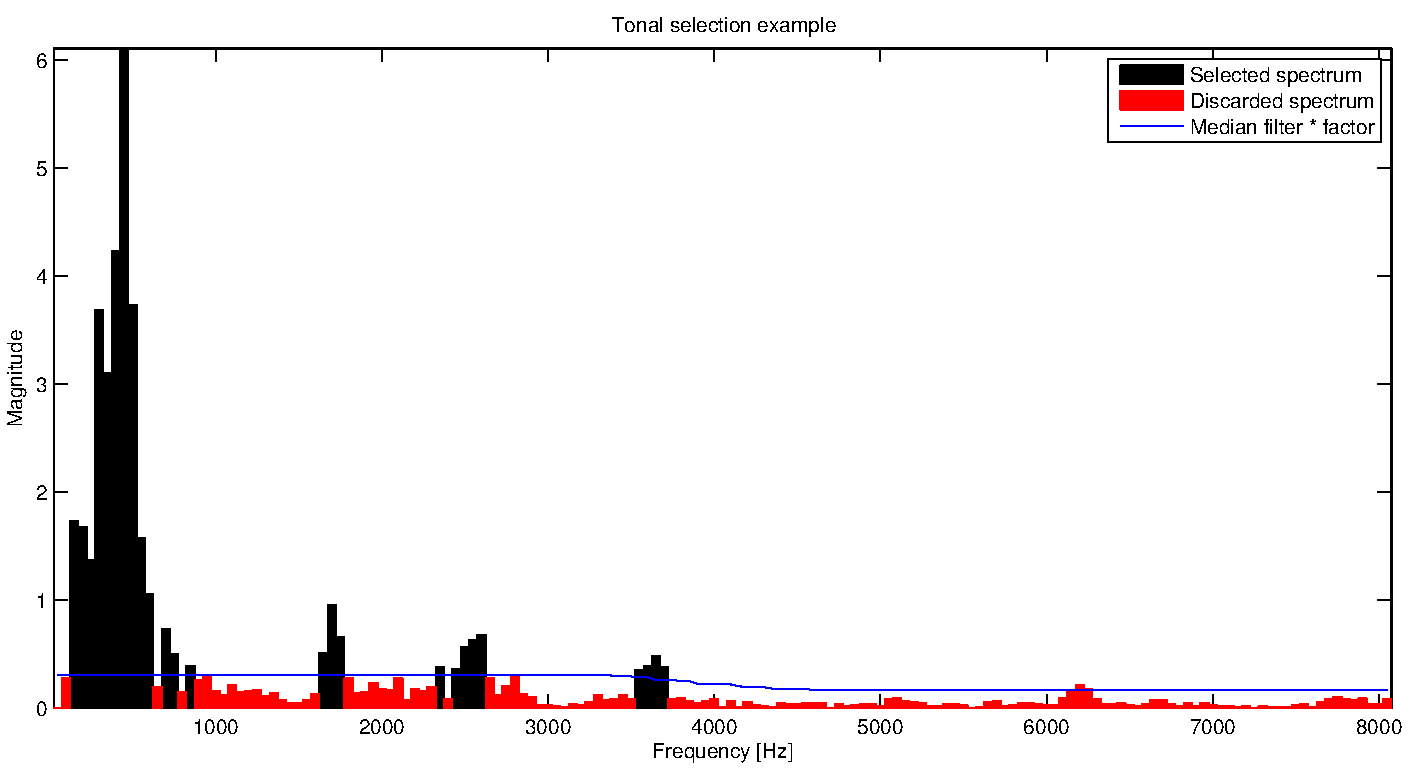
\includegraphics[width=14cm]{Separation_Spectrum_Selection.pdf}}
\end{minipage}
\caption{Example of the tonal selection algorithm. Block size of 320 samples. Audio sample rate of 16kHz.}
\label{fig:Separation_Spectrum_Selection.pdf}
\end{figure}

The algorithm proceeds by calculating a running median value of the STFT magnitude coefficients from a 320 sample long signal buffer. The media filter takes the running median value of 60 spectral samples and coefficients exceeding some factor $\nu$ of the median value (blue line in figure) are selected as tonal values (black bars). The red bars in Figure~\ref{fig:Separation_Spectrum_Selection.pdf} are assumed to be transient noise and their magnitude is set to zero. A suitable factor of the median value needs to be selected and for this application $\nu = 3.5$ was chosen. The detection of formant frequencies were additionally confined to be above 85 Hz and below 4000 Hz.

\begin{figure} %SeparationDiagram.pdf
\centering
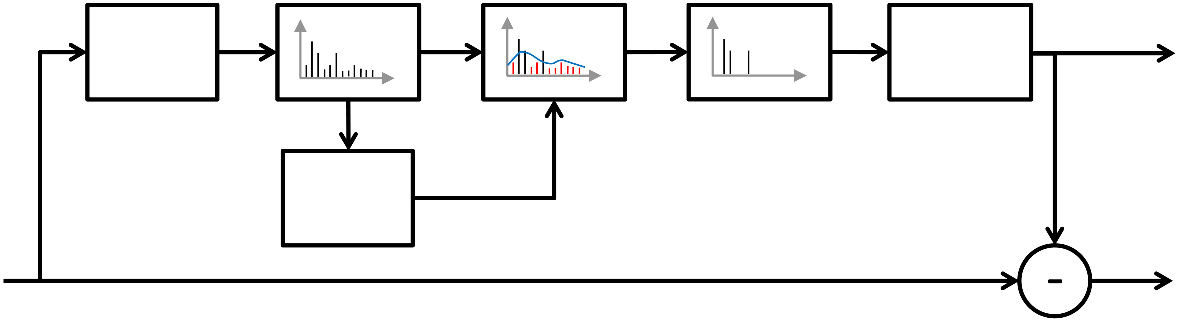
\includegraphics[width=140mm]{SeparationDiagram.pdf}
\begin{picture}(0,0)
\put(-420,20){Signal}
\put(-30,97){Tonal}
\put(-30,20){Residual}

\put(-302,45){Median}
\put(-302,30){filter}

\put(-362,88){STFT}
\put(-90,88){iSTFT}
\end{picture}
\caption{Diagram of separation algorithm.}
\label{fig:SeparationDiagram.pdf}
\end{figure}

\todo{This is a bit weak?}
A proposed addition to the algorithm described above and represented in Figure~\ref{fig:SeparationDiagram.pdf} includes a step to replace removed spectral information in frames suspected of being corrupted by key strokes to make the tonal component itself sound better. First of all a simple detection algorithm is employed to detect the spectral characteristics of an pulse. For the purpose of this implementation the detection criteria was a certain proportion of energy in a high frequency band in relation to a low frequency band, since energy in speech frames is largely located at the lower frequencies while pulses exhibit a wider frequency response. Figure~\ref{fig:SeparationDiagram2.pdf} shows a diagram of the revised algorithm. The removed spectral components in a corrupted frame is replaced by components from a historic buffer containing uncorrupted data.

\begin{figure} %SeparationDiagram2.pdf
\centering
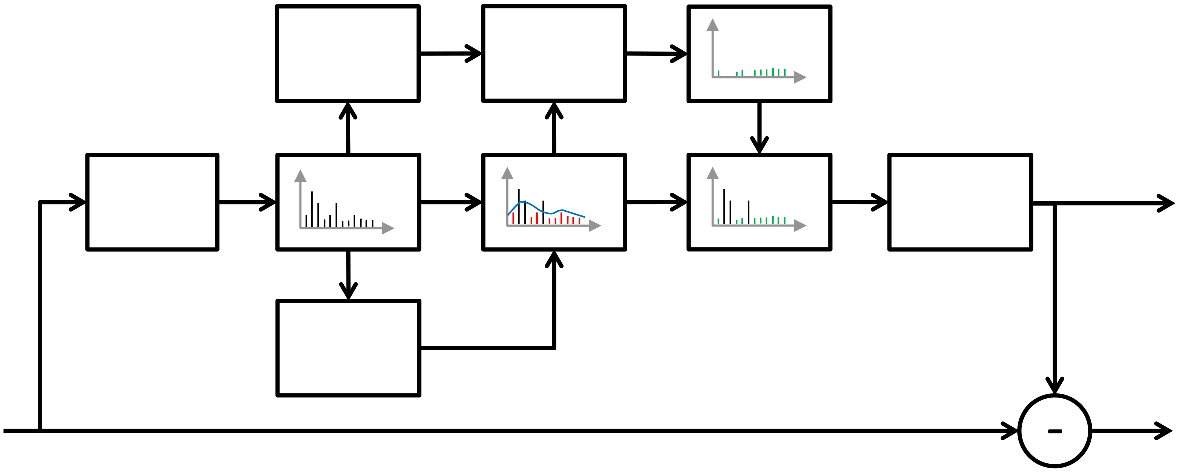
\includegraphics[width=140mm]{SeparationDiagram2.pdf}
\begin{picture}(0,0)
\put(-420,20){Signal}
\put(-30,97){Tonal}
\put(-30,20){Residual}

\put(-301,45){Median}
\put(-301,30){filter}

\put(-305,146){Simple}
\put(-305,131){Detector}

\put(-233,146){Vocal}
\put(-233,131){Memory}

\put(-362,88){STFT}
\put(-90,88){iSTFT}
\end{picture}
\caption{Diagram of separation algorithm.}
\label{fig:SeparationDiagram2.pdf}
\end{figure}


\subsection{Noise burst model}\label{sec:WPdetectionNB}
We assume that the coefficients for each terminal node $j$ can be modeled as some switched additive noise process such that:

\begin{equation}\label{eq:model1}
    w_{j}(n) = i_{n} \theta_{n,j} + v_{n,j},
\end{equation}
where $i_{n}$ is the binary (1/0) switching variable denoting the presence of $\theta_{n,j}$ for $i_{n} = 1$ and otherwise $i_{n} = 0$. The transient signal $\theta_{n,j}$ is thus a switched noise burst corrupted by additive noise $v_{n,j}$.
Note that the grouping of the transient noise bursts will depend on the statistics of $i_{n}$ so that it is most likely that detections occur clusters. could be modeled as a Markov chain which will describe some degree of cohesion between frequency and time, i.e. the transient noise pulses will typically have a similar index of onset and will likely stay active for a length of time proportional with wavelet scale $j$.

We can now express our model in terms of the additive noise and a matrix of coefficients

\begin{equation}\label{eq:model2}
\boldsymbol{w} = \boldsymbol{\theta} + \boldsymbol{v},
\end{equation}

where $\boldsymbol{w} = [\boldsymbol{w}_1,\boldsymbol{w}_2,\ldots,\boldsymbol{w}_J]$ and where $\boldsymbol{w}_j = [w_{1,j}, w_{2,j}, \ldots, w_{N,j}]^T$ for the $j$th set of coefficients. $\boldsymbol{\theta}$ is the corresponding switched noise burst $J$ by $N$ matrix containing elements $i_{n}\theta_{n,j}$ and $\boldsymbol{v}$ is the random additive noise describing, for example, the effect of speech on the coefficients. For simplicity we consider $i_{n}$ to be constant across scales $j$ so the discrete vector $\boldsymbol{i} = [i_{1}, i_{2}, \ldots, i_{N}]$ can take any one of $2^{N}$ values. It is although possible to let $i$ vary with $j$ to express different detection characteristics at different scales. The detection task now becomes the estimation of the true state of $\boldsymbol{i}$ from the observed sequence $\boldsymbol{w}$.

Assuming that both the noise burst $\boldsymbol{\theta}$ and the background noise $\boldsymbol{v}$ can be modeled as zero mean Gaussian distributions, we have that:

\begin{equation}\label{eq:burst}
\boldsymbol{\theta}_n \sim \mathcal{N}_{\boldsymbol{\theta}_n}(0,\Lambda),
\end{equation}

where $\Lambda$ is a covariance matrix, here taken as diagonal with diagonal elements $\left[\lambda_{1}, \lambda_{2}, \ldots, \lambda_{J}\right]$, learned from training examples of keyboard clicks.

The background noise is also modelled as a zero-mean Gaussian process so that:

\begin{equation}\label{eq:noise}
\boldsymbol{v}_n \sim \mathcal{N}_{\boldsymbol{v}_n}(0,C_{\boldsymbol{v}}),
\end{equation}

where again $C_v$ is a diagonal covariance matrix with diagonal components \\*$[\sigma_{v,1}^2, \sigma_{v,2}^2, \ldots, \sigma_{v,J}^2]$.

%Bayes'
Treating the detection state $\boldsymbol{i}$ as a discrete random vector the probability of $\boldsymbol{i}$ conditional upon the observed (and corrupted) data $\boldsymbol{w}$ and other prior information available to us. This posterior probability $p(\boldsymbol{i}|\boldsymbol{w})$ can be expressed using Bayes' rule so that

\begin{equation}\label{eq:Bayes}
p(\boldsymbol{i}|\boldsymbol{w}) = \frac{p(\boldsymbol{w}|\boldsymbol{i})p(\boldsymbol{i})}{p(\boldsymbol{w})}
\end{equation}

where the likelihood $p(\boldsymbol{w}|\boldsymbol{i})$ will be a significant component of $p(\boldsymbol{i}|\boldsymbol{w})$.
$\boldsymbol{\theta}$ is our switched random noise process and its amplitude is defined by the noise burst amplitude p.d.f. $p_{\boldsymbol{\theta}}$ which is the joint distribution for the burst amplitudes where $i_{n} = 1$.

Since both functions $p_{\boldsymbol{v}}(\boldsymbol{v})$ and $p_{\boldsymbol{\theta}}(\boldsymbol{\theta})$ are zero-mean Gaussians, we can express each set of wavelet coefficients as $w_j(n)$ as:

\begin{equation}\label{eq:cases}
  w_j(n) \sim
  \begin{cases}
    \mathcal{N}(0,\sigma_{v,j}^2 + \lambda_j), & \quad i_n = 1\\
   \mathcal{N}(0,\sigma_{v,j}^2), & \quad i_n = 0,
  \end{cases}
\end{equation}

and the likelihood function $p(\boldsymbol{w}|\boldsymbol{i})$ becomes

\begin{equation}\label{eq:likelihood1}
p(\boldsymbol{w}|\boldsymbol{i}) = \prod^J \prod^N \mathcal{N}(0,\sigma_{v,j}^2 + i_n\lambda_j).
\end{equation}

The Maximum Likelihood (ML) estimate for $i_n$ can now trivially be calculated as
\begin{equation}\label{eq:ml1}
\hat{i}_n^{\textrm{MLE}} = \arg\max_{i\in\{0,1\}} \prod^J \mathcal{N}(0,\sigma_{v,j} + i_n\lambda_j).
\end{equation}

Given that keyboard transient noise usually occurs in long bursts, it is essential to incorporate this knowledge into the model. We thus model the state vector $\boldsymbol{i}$ as a Hidden Markov Model (HMM). Decoding of the hidden state sequence can then be computed using the Viterbi algorithm\cite{Viterbi1967}\cite{Forney1973} to calculate the most likely detection sequence $\boldsymbol{i}$:

\begin{equation}\label{eq:viterbi}
\hat{\boldsymbol{i}}^{\textrm{MAP}} = \arg\max_{{\bf i}\in\{0,1\}^N} p(i_{0})\prod_n p(i_n | i_{n-1})p(\boldsymbol{w}(n) | i_n).
\end{equation}

Here $p(i_{0})$ is the starting probability, $p(i_n | i_{n-1})$ is the transition probability from one state to the next and $p(\boldsymbol{w}(n) | i_n)$ is the emission probability or the observation probability, as determined by (\ref{eq:cases}).

The algorithm proposed above aims to implement a detection algorithm with superior temporal resolution compared with current approaches and to view the detection state as an HMM in order to incorporate prior knowledge of the likely evolution of the detection state. In addition, the proposed algorithm is also fundamentally different from current approaches in that it utilises a sparse residual signal that is well modelled by a wavelet basis.

\subsection{AR filtering approach}\label{sec:WPdetectionAR}

The terminal node coefficients of the WPT of an incoming audio sequence $x(n)$ of length $N$ is defined as $X(j,t)$ where $X_j$ is the $j$th terminal node, $j \in \{1, \ldots, J\}$, and $t$ is the time index related to $n$. A level $L$ WPT gives $J = 2^L$ terminal nodes. $X(t)$ will be used to denote a vector of all coefficients at a given time index $t$. We assume that the coefficients for each terminal node $j$ follow this linear predictive model

\begin{equation}\label{eq:lpm}
X(j,t) = \sum_{m=1}^{M} a_{j,m} X(j,t - m) + v(j,t),
\end{equation}

where $a_{jm}$ is the $m$th weight applied to the $j$th terminal node so that $\mathbf{a}_j = \{a_{j,1}, \ldots, a_{j,M} \}$, $M$ is the size of the buffer used, and $v(j,t)$ is Gaussian noise with zero mean so that

\begin{equation}\label{eq:lpmnoise}
v(j,t) \sim \mathcal{N}_v(0,\sigma^2_{j,t}).
\end{equation}

We can now express the probability of $X(j,t)$ conditional on prior values of $X$.

\begin{align}\label{eq:likelihood}
p\left(X\left(j,t\right)|X\left(j,t-1\right),\ldots,X\left(j,t-M\right)\right) = \nonumber\\
\qquad \mathcal{N}_X\left( \sum_{m=1}^M a_{j,m} X(j,t - m), \sigma_{j,t}^2\right),
\end{align}

and the marginal probability can be expressed as

\begin{equation}\label{eq:marginal}
p\left(X(t)\right) = \prod^J p\left(X(j,t)\right),
\end{equation}

assuming that the conditional probabilities for each set of coefficients are independent.

We can now calculate the log-likelihood $\log\mathcal{L} = \log{p\left(X(t)\right)}$ for the current coefficient $X(t)$,

\begin{align}\label{eq:loglike}
\log \mathcal{L} &= \log \left\{ \prod^J p \left( X(j,t) | X(j,t-1),\ldots,X(j,t-M) \right) \right\} \\
&=  \sum^J \log \left\{p \left( X(j,t) | X(j,t-1),\ldots,X(j,t-M) \right) \right\}\nonumber\\
&=  -\frac{1}{2} \sum^J \frac{1}{\sigma_{j,t}^2}\left(X(j,t) -  \sum_{m=1}^{M} a_{j,m} X(j,t - m) \right)^2 + C_{j,t}\nonumber,
\end{align}
where $C_{j,t}$ is a constant. The value $\log \mathcal{L}$ is now a measure of how well $X(t)$ can be predicted by its previous values.

\section{Methods}\label{sec:WPmethods} %A note about the issues of plotting/decribing/comparing detection results.
\subsection{Separation algorithm}
Results provided for the separation algorithm mainly take the form of waveforms. These provide a reference for the amplitude reduction achieved for speech segments of the signal containing both speech and keyboard strokes. Figures are also provided that show the effect of the separation algorithm on both a clean speech segment as well as a keyboard stroke corrupted segment.

A plot of a moving frame estimate of the Mean Squared Error (MSE) is also provided as well as other error measurements such as Peak Signal to Noise Ration (PSNR) and the maximum MSE for the entire signal.

\subsection{Detection algorithms}
The goal of any validation of a detection algorithm should clearly be to assess whether or not the algorithm detects what it is designed to detect as well as if it can dismiss everything else. In Section~\ref{sec:WPdata} it was noted that the pulses in question contain multiple segments that vary in length, amplitude and structure in some cases. To assess the performance of the detection algorithm having a complete record of time of the pulse occurrence would clearly be advantageous. While the primary goal of a keyboard is to inform the computer of keystrokes and their timing, the sample rate of a keyboard is often nowhere near that of audio. A standard desktop keyboard is quoted as accepting 1000 keystrokes per minute based on internal testing\cite{MSCurveKeyboard3000}. In addition to this comes additional variable latency inherent in the OS ultimately rendering any such data useless. To achieve a suable ground truth estimate of keyboard strokes within audio files manual labeling is the only viable option and this procedure gives rise to a range of additional problems and sources of error:

\begin{itemize}
  \item Variability in the marking of the pulse onset due to subjective factors.
  \item Pulses hidden within speech segments can appear invisible yet audible with few audible cues to their exact temporal location.
  \item Ambiguity in the number of pulse onsets within a single keystroke event as seen in Figure~\ref{fig:KeyboardStrokeSlow}.
\end{itemize}

Especially the latter concern has caused a variety of issues in relation to the meaningful evaluation of the detection performance of all evaluated detection algorithms within this chapter. While a typical keyboard stroke can contain multiple pulses at varying delays from each other, other background pulses might well also be of interest when considering a detection algorithm for audio restoration. While not the primary target, mouse clicks and foot steps from other sources might exhibit many of the spectral characteristics of keyboard strokes and hence cause a similar level of nuisance.

To evaluate the performance of the detection algorithms in this section, a library of audio files have been used divided into 3 main categories.

\begin{description}
  \item[Speech] Speech segments of 1-2 seconds manually verified to contain nothing that should be considered a noise pulse.
  \item[Keyboard strokes] Audio segments containing nothing but a keyboard stroke.
  \item[Mixed] Speech segment containing a keyboard stroke.
\end{description}

The speech segments serve as a reference for the false detection rate, the keyboard stroke files provide an unambiguous reference for positive detections and the mixed files are mainly of interest for either visual and audible inspections and subjective restoration trials conducted in the following chapter.

The term \emph{false detection} will be used to refer to an algorithm wrongfully indicating the presence of a noise pulse when a different cause of the detection can be verified. Typically this would be the sharp onset of a speech segment or a loud speech in general. A \emph{correct detection} is generally anything else than a \emph{false detection}. This again outlines the difficulty of assessing a noise detection algorithm and great care must be taken when generating speech sequences for \emph{false detection} rate calculations to not allow anything in the signal that could rightly be considered transient or impulsive noise.

The 4 main detection methods tested in the following section are:
\begin{enumerate}
  \item Noise burst model from section~\label{sec:WPdetectionNB}
  \item AR filter method from section~\label{sec:WPdetectionAR}
  \item UKD algorithm from \cite{Subramanya2007}
  \item Generic median filter detector.
\end{enumerate}
Both of the methods outlined in this chapter will utilize the pre-processing stage discussed in section~\label{sec:WPdetectionSep}.

While the AR filter, UKD and median filter methods all rely on the thresholding on some statistical or detection value, the Noise burst model relies on a range of parameters such as variance estimates and transition probabilities. Since the sensitivity, and thereby detection and false detection rate, are dependent on these thresholds a method for visualising the performance of the algorithms is to compare the range of these statistical or detection values that the thresholds apply to. The greater the margin between false detections and correct detections the stronger the detection capability of the algorithm.

The Noise burst model will be compared to other algorithms by calibrating the sensitivity of all algorithms to a similar standard of sensitivity using clean speech data and making sure nothing is detected within them.

While the noise burst model offers a statistical framework for estimating the duration of pulses, it is also possible to assume the length of a corruption based on experience or even estimate the extent of the corruption based on the level of the excitation over the threshold. This approach will be assumed on all other algorithms and therefore short detections extents in future sections will not necessarily be considered undesirable.

\section{Results}\label{sec:WPresults}
\subsection{Separation Results} %DONE
Figure~\ref{fig:Separation_Residual_Example} shows an example of the residual obtained by simply subtracting outstanding peaks from the spectrum on frames of 20ms with 10ms overlap. The spectral peaks were identified using a threshold of a factor of three of the median filtered spectrum excluding frequencies below 85 Hz and above 10 kHz. The audio data presented in Figure~\ref{fig:Separation_Residual_Example} is a short sentence with two keystrokes embedded in it. The red plot overlay shows the residual where it is clear that the speech magnitude has been greatly reduced while the two clear keystrokes are largely left unchanged. \todo{Numerical justification for the effectiveness of the separation.}

\begin{figure}
\begin{minipage}[b]{1.0\linewidth}
  \centering
  \centerline{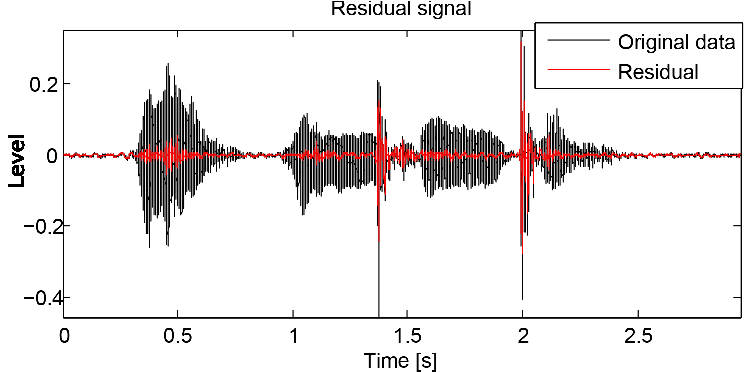
\includegraphics[width=10cm]{Separation_Residual_Example}}
\end{minipage}
\caption{Example of the separation step.}
\label{fig:Separation_Residual_Example}
\end{figure}

An example of the waveforms from the separation processing stage with both the tonal and the residual component zoomed in on a keyboard stroke plotted together, can be seen in Figure~\ref{fig:SeparationWaveformEx320.pdf}a and Figure~\ref{fig:SeparationWaveformEx320.pdf}b respectively. The data displayed in Figure~\ref{fig:SeparationWaveformEx320.pdf} is processed by applying the separation algorithm over blocks of 320 samples and sampled at 16kHz which is equivalent to blocks of 20ms, a common block size in communication systems\cite{Subramanya2007}. While the separation stage clearly removes the initial pulse, a strong tonal component of the keyboard typing pulse is retained and a lower frequency pulse, presumably related to the keyboard stroke, is also retained later in the example.

\begin{figure} %SeparationWaveformEx320.pdf
\begin{minipage}[b]{1.0\linewidth}
  \centering
  \centerline{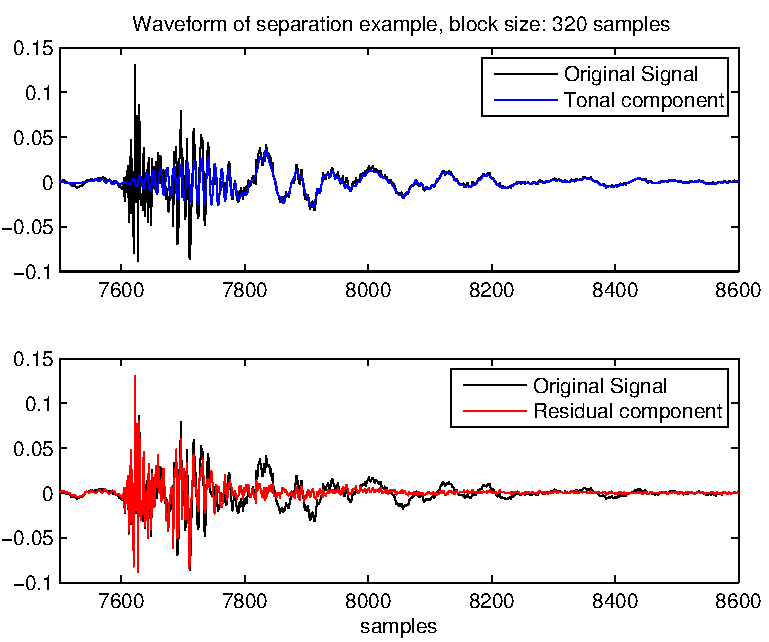
\includegraphics[width=12cm]{SeparationWaveformEx320.pdf}
  \begin{picture}(0,0)
\put(-310,270){a)}
\put(-310,130){b)}
\end{picture}}
\end{minipage}
\caption{Separation example of keyboard pulse, a) Tonal component, b) residual component. Sample rate: 16kHz. Block size: 320.}
\label{fig:SeparationWaveformEx320.pdf}
\end{figure}

Applying the algorithm to block sizes of 640 samples yields a better separation result for short tonal components as seen in Figure~\ref{fig:SeparationWaveformEx640.pdf}. Within blocks of 320 samples the tonal components of keyboard pulses may contain enough energy to make a significant impression on the spectrum to be detected as a tonal component but with a block size of 640 samples it is clear that less of the energy introduced by the keyboard stroke is retained.

\begin{figure} %SeparationWaveformEx640.pdf
\begin{minipage}[b]{1.0\linewidth}
  \centering
  \centerline{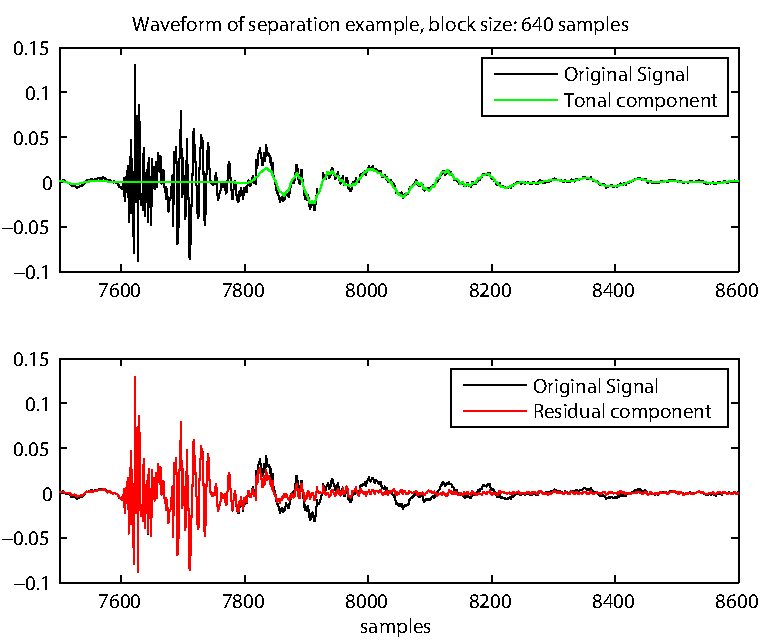
\includegraphics[width=12cm]{SeparationWaveformEx640.pdf}
  \begin{picture}(0,0)
\put(-310,270){a)}
\put(-310,130){b)}
\end{picture}}
\end{minipage}
\caption{Separation example of keyboard pulse, a) Tonal component, b) residual component. Sample rate: 16kHz. Block size: 640.}
\label{fig:SeparationWaveformEx640.pdf}
\end{figure}

In Figure~\ref{fig:SeparationWaveformExBig320.pdf} and \ref{fig:SeparationWaveformExBig640.pdf} a the keyboard strokes from Figure~\ref{fig:SeparationWaveformEx320.pdf} and \ref{fig:SeparationWaveformEx640.pdf} are seen with speech data. For both block sizes it is seen that the voiced parts of the signal are mainly represented in the tonal component while the keyboard stroke, around sample number 7600, is largely within the residual component.

\begin{figure} %SeparationWaveformExBig320.pdf
\begin{minipage}[b]{1.0\linewidth}
  \centering
  \centerline{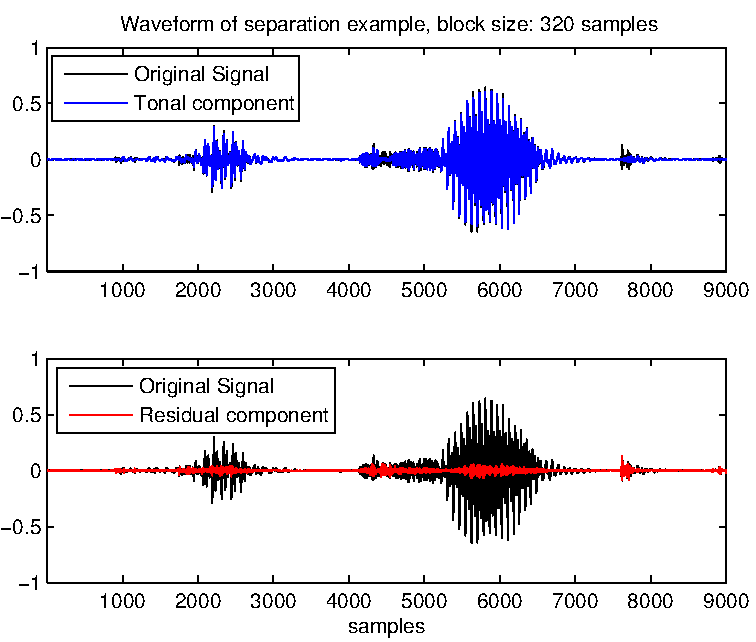
\includegraphics[width=12cm]{SeparationWaveformExBig320.pdf}
  \begin{picture}(0,0)
\put(-310,275){a)}
\put(-310,135){b)}
\end{picture}}
\end{minipage}
\caption{Separation example of speech and pulses, a) Tonal component, b) residual component. Sample rate: 16kHz. Block size: 320.}
\label{fig:SeparationWaveformExBig320.pdf}
\end{figure}

\begin{figure} %SeparationWaveformExBig640.pdf
\begin{minipage}[b]{1.0\linewidth}
  \centering
  \centerline{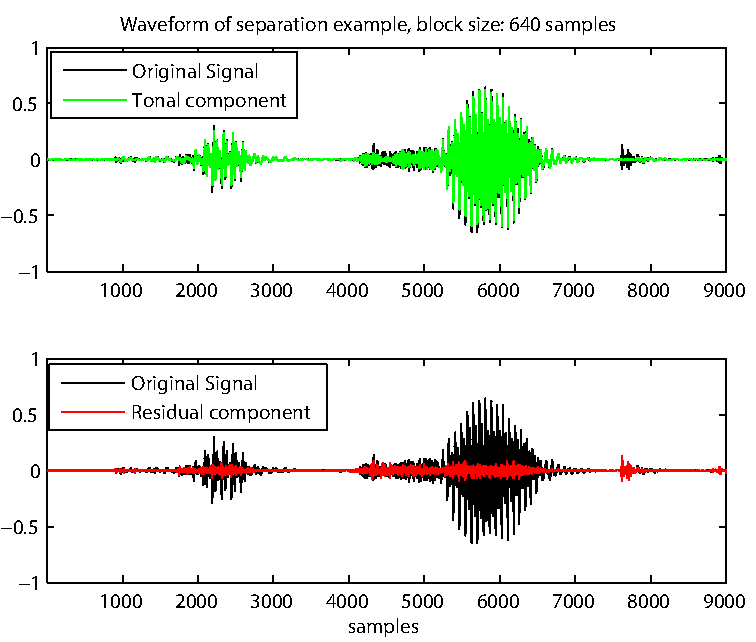
\includegraphics[width=12cm]{SeparationWaveformExBig640.pdf}
  \begin{picture}(0,0)
\put(-310,275){a)}
\put(-310,135){b)}
\end{picture}}
\end{minipage}
\caption{Separation example of speech and pulses, a) Tonal component, b) residual component. Sample rate: 16kHz. Block size: 640.}
\label{fig:SeparationWaveformExBig640.pdf}
\end{figure}

To further evaluate the effect of the separation algorithm a comparison of the MSE and the waveform is provided in Figure~\ref{fig:SeparationError.pdf}. In Figure~\ref{fig:SeparationError.pdf}(a) the corrupted signal and the tonal component of the corrupted signal is compared to the original uncorrupted signal. This comparison is made possible since the noisy signal has been corrupted by the linear addition of a keyboard stroke and therefore a perfect record of the uncorrupted signal is available for the MSE estimate. The large spike in Figure~\ref{fig:SeparationError.pdf}(a) is the location of the corruption in the signal and it is clearly noted how both the corrupted signal as well as the tonal component of the corrupted signal excites the MSE estimate to varying degrees.

Figure~\ref{fig:SeparationError.pdf}(b) shows the waveform for the signals compared in Figure~\ref{fig:SeparationError.pdf}(a) and Figure~\ref{fig:SeparationErrorData.pdf} provides a zoomed in view of the waveform for a further detailed comparison.

For the audio segment in Figure~\ref{fig:SeparationError.pdf} in addition to the MSE estimate provided, the Peak Signal to Noise Ratio (PSNR) value was also increased from \todo{Recalculate PSNR} 80.5 dB, for the corrupted signal, to 82 dB for the tonal component of the corrupted signal. The maximum MSE was also calculated to be reduced from 0.52 to 0.32 for the entire signal.

\begin{figure} %SeparationError.pdf
\begin{minipage}[b]{1.0\linewidth}
  \centering
  \centerline{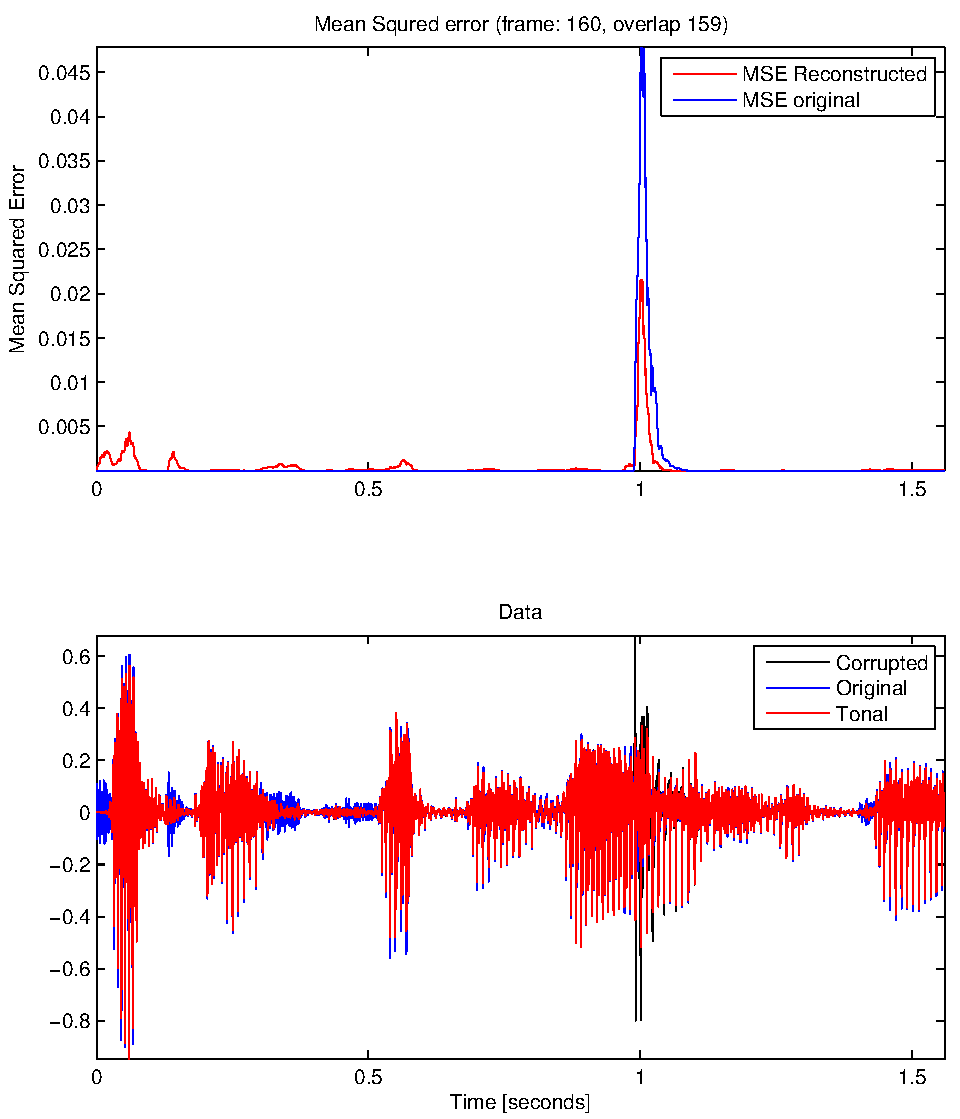
\includegraphics[width=12cm]{SeparationError.pdf}
  \begin{picture}(0,0)
\put(-310,390){(a)}
\put(-310,180){(b)}
\end{picture}}
\end{minipage}
\caption{Separation performance example of speech and an pulse, (a) Means Squared Error (MSE) comparison (b) waveform comparison. Sample rate: 16kHz. Block size: 640.}
\label{fig:SeparationError.pdf}
\end{figure}

\begin{figure} %SeparationErrorData.pdf
  \centering
  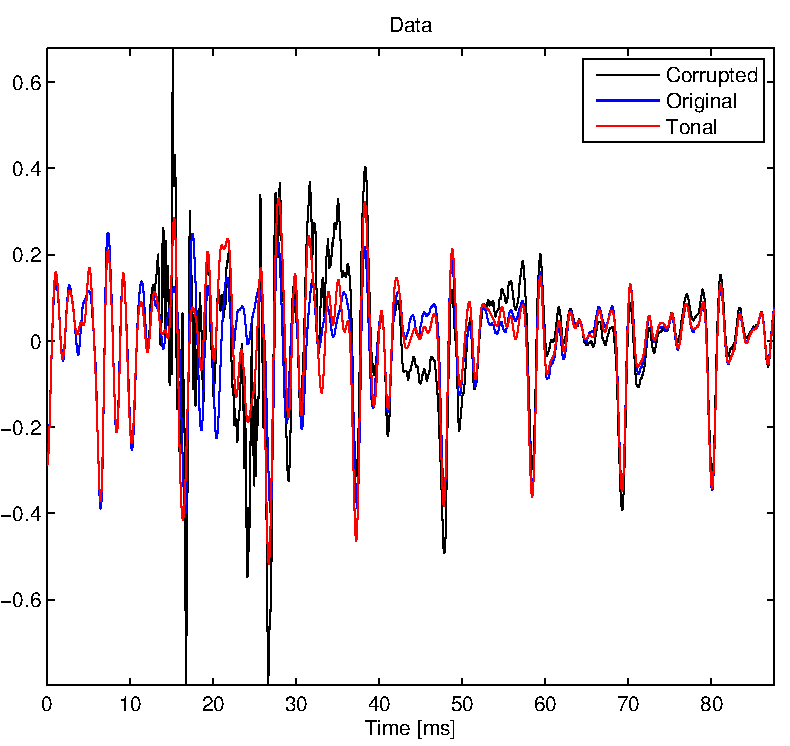
\includegraphics[width=10cm]{SeparationErrorData.pdf}
\caption{Zoomed in version of the waveform from Figure~\ref{fig:SeparationError.pdf}. Sample rate: 16kHz. Block size: 640.}
\label{fig:SeparationErrorData.pdf}
\end{figure}


\subsection{Noise Burst method results}\label{sec:WPdetectionNBresults}
%Introduction to results
The performance of the detection algorithm proposed (red) is in this chapter compared to two other keystroke detection algorithms. The first algorithm is the Unsupervised Keystroke Detection (UKD) algorithm presented in \cite{Subramanya2007} (blue), and the second is a standard median filtered algorithm (green) $y(n) = x(n)^2 - \textrm{MED}\left|x(n)^2\right|$ where $x(n)$ is the incoming signal, $y(n)$ is the detection statistics and $\textrm{MED}\left|\cdot \right|$ is the median filter. The following data is all sampled at 32 kHz and recorded either on a laptop or a microphone attached near an external PC keyboard. The median filter buffer is 10 samples and the UKD algorithm is implemented as described in \cite{Subramanya2007}.

Figure~\ref{fig:NBDetCompare.pdf} shows an example of the detection algorithms running on the same audio sequence used in Figure~\ref{fig:Separation_Residual_Example}. The coloured step functions indicate a detection with their high state and no detection with their low state. All algorithms have been tuned to be as sensitive as possible while only allowing correct detections, or plausibly correct detections. Lowering the thresholds on the UKD and the median filter algorithms slightly would cause a false detection in this example. In this example the Noise Burst model quite clearly picks out the keystroke pulse and a secondary pulse associated with the lifting of the keyboard key. It is also clearly seen how the HMM stage estimates the most likely length of the pulse and not just the onset as the UKD and median filter approaches.

\begin{figure} %NBDetCompare.pdf
\begin{minipage}[b]{1.0\linewidth}
  \centering
  \centerline{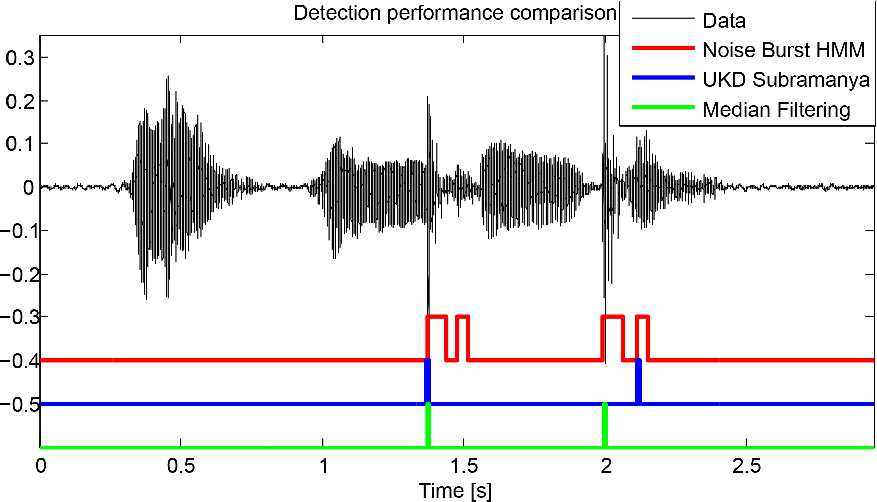
\includegraphics[width=12cm]{NBDetCompare.pdf}
  \begin{picture}(0,0)
%\put(-310,275){a)}
%\put(-310,135){b)}
\end{picture}}
\end{minipage}
\caption{Comparison of Noise Burst detection algorithm on mixed signal.}
\label{fig:NBDetCompare.pdf}
\end{figure}

To quantify the performance of the algorithms, the test performed in \ref{fig:NBDetCompare.pdf} was run on the two audio sequences seen in Figure~\ref{fig:NBDetectionResults}. Figure~\ref{fig:NBDetectionResults}(a) shows the results from running the algorithm on 10 clean keystrokes, and Figure~\ref{fig:NBDetectionResults}(b) shows the results from 10 keystrokes but each of which are embedded at different points in different utterances. Both the Noise Burst model and the UKD algorithm manages to pick up all 10 keystrokes, with UKD catching some additional faint pulses, while the median filter misses 3 keystrokes, mainly the ones with the smallest maximum amplitude. The median filter misses all but 2 keystrokes in Figure~\ref{fig:NBDetectionResults}(b), while the UKD algorithm and the noise burst algorithm misses 3 and 1 respectively. The stars in Figure~\ref{fig:NBDetectionResults}(b) indicate the ground truth, or in other words the best estimate of where the initial keystroke occurred in the sequence. The algorithms are all tuned to be as sensitive as possible on a third audio sequence containing 8 seconds of only speech without getting any detections.

\begin{figure}
\begin{minipage}[b]{1.0\linewidth}
  \centering
  \centerline{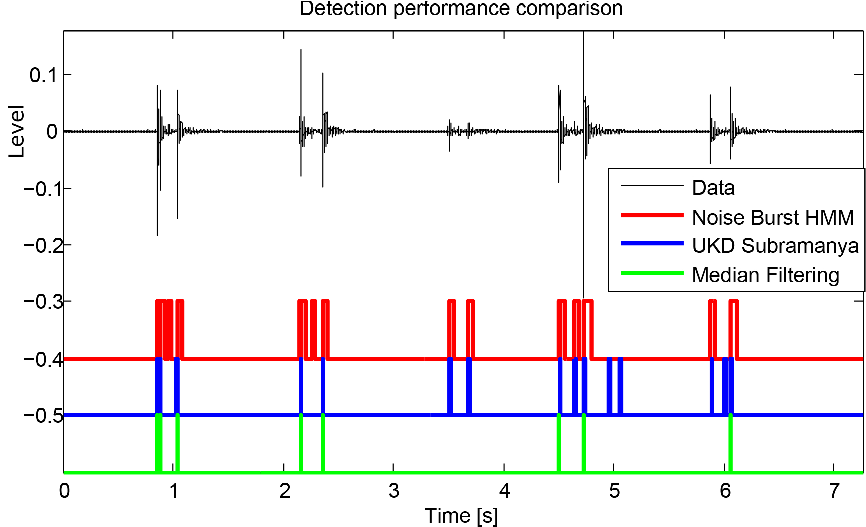
\includegraphics[width=12.5cm]{NBDetCompareLongTaps}}
%  \vspace{2.0cm}
  \centerline{(a) 10 taps with no speech.}\medskip
\end{minipage}
%
\begin{minipage}[b]{1.0\linewidth}
  \centering
  \centerline{\includegraphics[width=12.5cm]{NBDetCompareLongTapsnTalk}}
%  \vspace{1.5cm}
  \centerline{(b) 10 taps embedded in 10 utterances. Stars indicate ground truth.}\medskip
\end{minipage}
\hfill
%
\caption{Detection results for sequences of taps.}
\label{fig:NBDetectionResults}
\end{figure}

\subsubsection{False detection rate}
To further quantify the performance of the algorithm a similar test to the above was run on 61 seconds of speech and 43 individual keyboards taps. The audio was recorded via an external microphone in 16kHz and all algorithms were tuned similarly to the previous test. The results of this test has been tabulated in Table~\ref{table:NBResultsTest}.

\begin{table}
\caption{Detection results}
\centering
\begin{tabular}{|l | c c c|}
\hline
                            & Noise Burst   & UKD       & Median        \\
 \hline
 Correct detection rate     & 34 \%         & 20 \%     & 50 \%         \\
 False detections pr second & 0             & 0.03      & 0.02          \\
 \hline
 \end{tabular}
 \label{table:NBResultsTest}
\end{table}

\subsection{AR Filter method results}
Figure~\ref{fig:ARFilterDetectionResults} shows, similar to Figure~\ref{fig:NBDetectionResults}, the detection performance for the AR filter method (red) in relation to that of the UKD\cite{Subramanya2007} (blue) and the standard median filter method (green). Figure~\ref{fig:ARFilterDetectionResults}(a) shows the algorithms performance on 10 clean keyboard strokes while Figure~\ref{fig:ARFilterDetectionResults}(b) shows an example of the algorithms' performance when the keyboard strokes are embedded in speech. As can be seen in Figure~\ref{fig:NBDetectionResults} with the proposed noise burst model, the AR filter model in Figure~\ref{fig:ARFilterDetectionResults} indicates a detection in between the first and the second correct detections. Both of these detections are clearly provoked by the sudden onset of the speech utterance and is considered a false detection.

\begin{figure}
\begin{minipage}[b]{1.0\linewidth}
  \centering
  \centerline{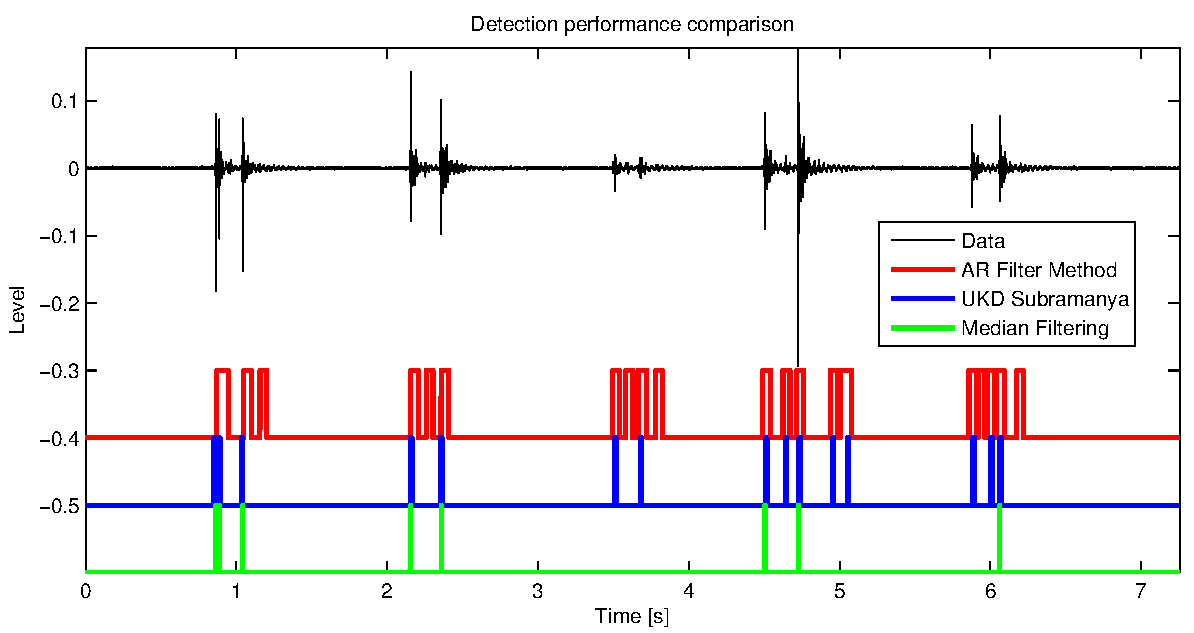
\includegraphics[width=12.5cm]{ARFiltCompareLongTaps.pdf}}
%  \vspace{2.0cm}
  \centerline{(a) 10 taps with no speech.}\medskip
\end{minipage}
%
\begin{minipage}[b]{1.0\linewidth}
  \centering
  \centerline{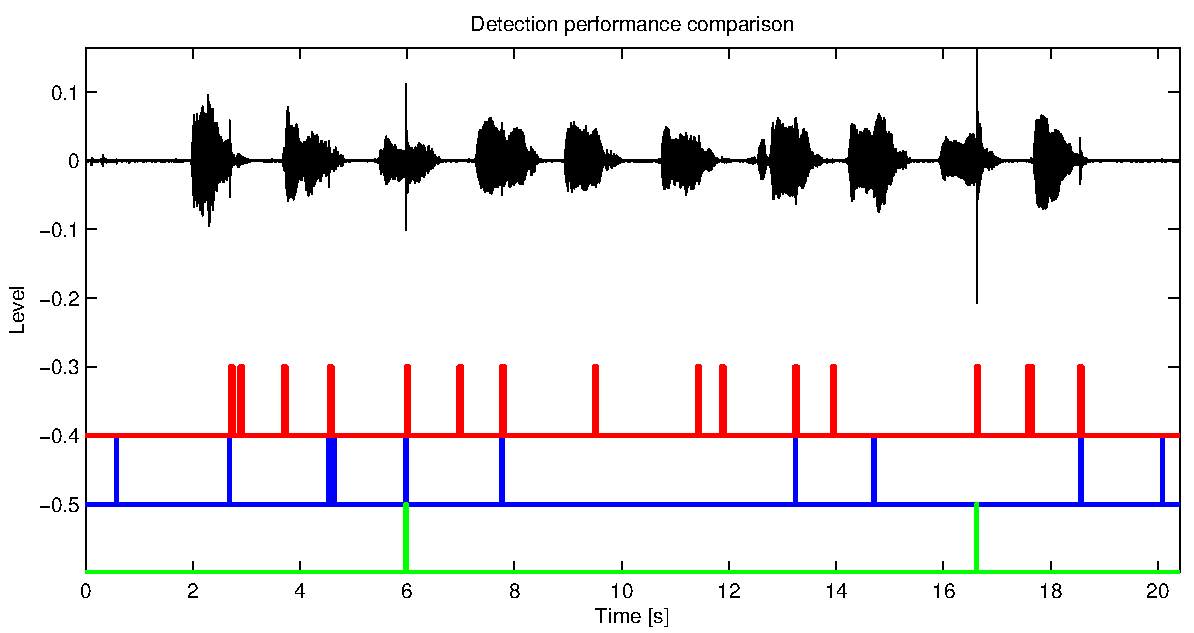
\includegraphics[width=12.5cm]{ARFiltCompareLongTapsnTalk.pdf}}
%  \vspace{1.5cm}
  \centerline{(b) 10 taps embedded in 10 utterances. Stars indicate ground truth.}\medskip
\end{minipage}
\hfill
%
\caption{Detection results for sequences of taps.}
\label{fig:ARFilterDetectionResults}
\end{figure}

Since the 3 detection methods compared in this section all work by thresholding some statistical value the maximum excitation for various signal types can be compared and ideally there should be a margin between correct detection and false detections in which a threshold limit can be set. Figures~\ref{fig:DetectPerfARFilt.pdf} - \ref{fig:DetectPerfMedian.pdf} are figures showing the maximum excitations for 40 different keystroke files and 53 different speech segments for the three different detection methods previously compared in this section. Figures~\ref{fig:DetectPerfARFilt.pdf} and \ref{fig:DetectPerfUKD.pdf} show that for both the AR filter and the UKD method, there is a distinct margin in between the lowest maximum excitation for a positive detection and the highest maximum detection for a false detection indicating that there are a range of values for which perfect detection could be achieved for this training set. The minimum response for correct detection is 1067 and 91.4 while the maximum response for a false detection, or for the clean speech segments, is 714.4 and 72.2 for the AR filter and UKD methods respectively. In relative terms the maximum response for a false detection in this test would be 67\% of the minimum correct detection response while the same number for the UKD method would be 79\%.
Figure~\ref{fig:DetectPerfMedian.pdf} shows that although the mean value for the maximum detection statistics are clearly separated, several samples give results within the range of 0.05, the lowest maximum detection for a keystroke, and 0.29, the highest maximum detection for a clean speech signal.

\begin{figure} %DetectPerfARFilt.pdf
\begin{minipage}[b]{1.0\linewidth}
  \centering
  \centerline{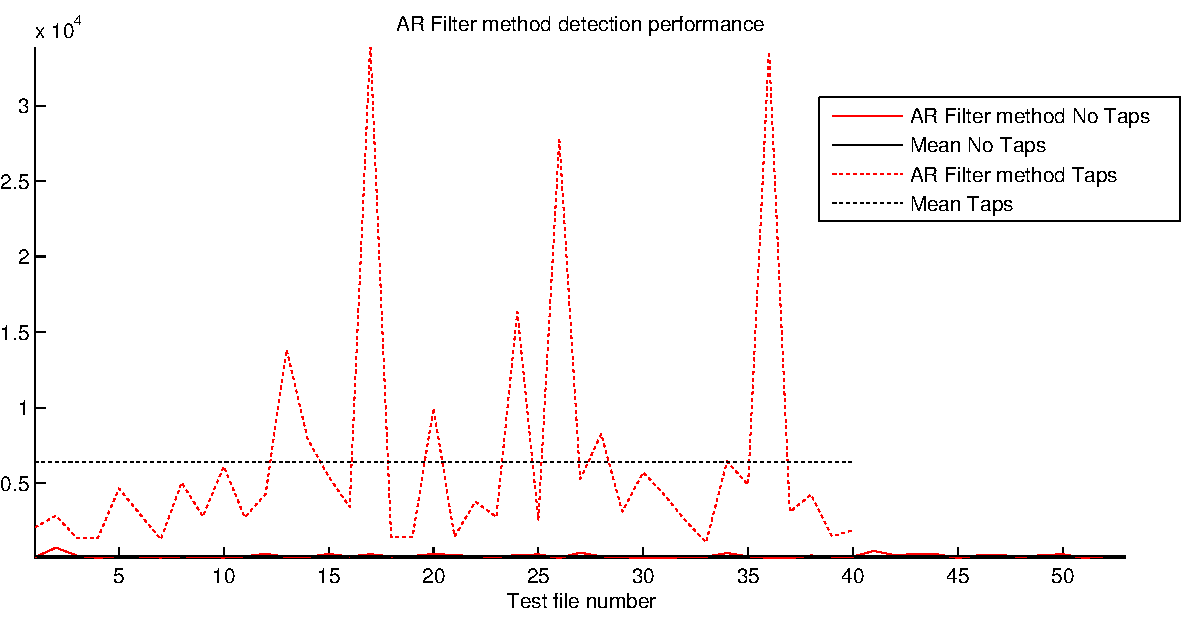
\includegraphics[width=12cm]{DetectPerfARFilt.pdf}
  \begin{picture}(0,0)
%\put(-310,275){a)}
%\put(-310,135){b)}
\end{picture}}
\end{minipage}
\caption{Maximum detector response for files with either a tap or some speech.}
\label{fig:DetectPerfARFilt.pdf}
\end{figure}

\begin{figure} %DetectPerfUKD.pdf
\begin{minipage}[b]{1.0\linewidth}
  \centering
  \centerline{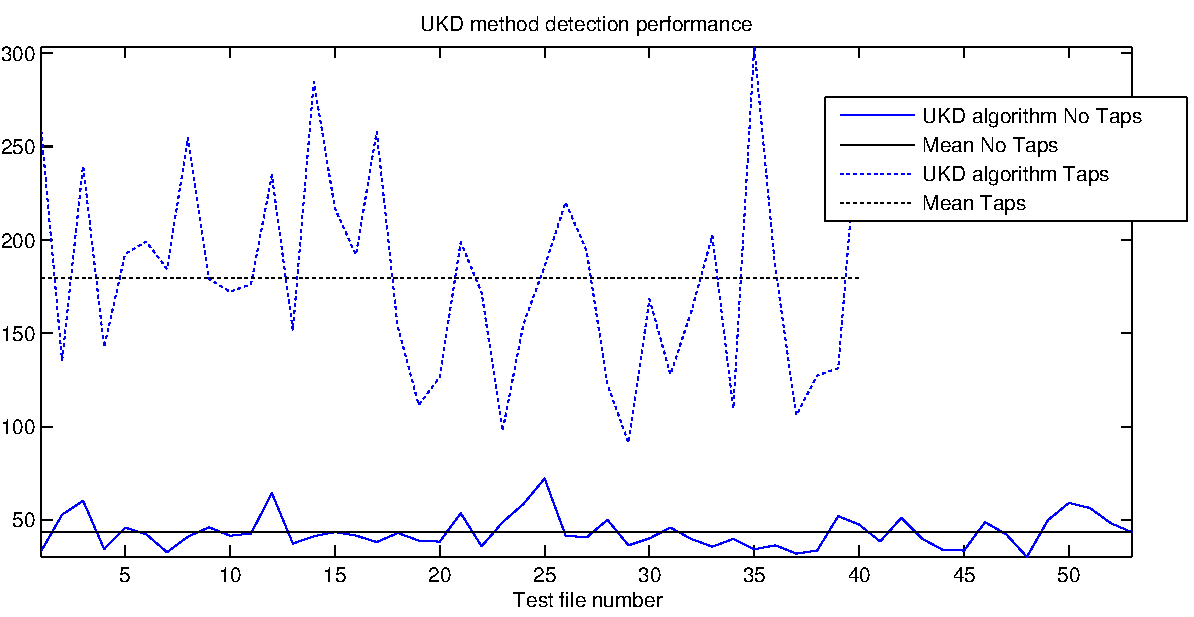
\includegraphics[width=12cm]{DetectPerfUKD.pdf}
  \begin{picture}(0,0)
%\put(-310,275){a)}
%\put(-310,135){b)}
\end{picture}}
\end{minipage}
\caption{Maximum detector response for files with either a tap or some speech.}
\label{fig:DetectPerfUKD.pdf}
\end{figure}

\begin{figure} %DetectPerfMedian.pdf
\begin{minipage}[b]{1.0\linewidth}
  \centering
  \centerline{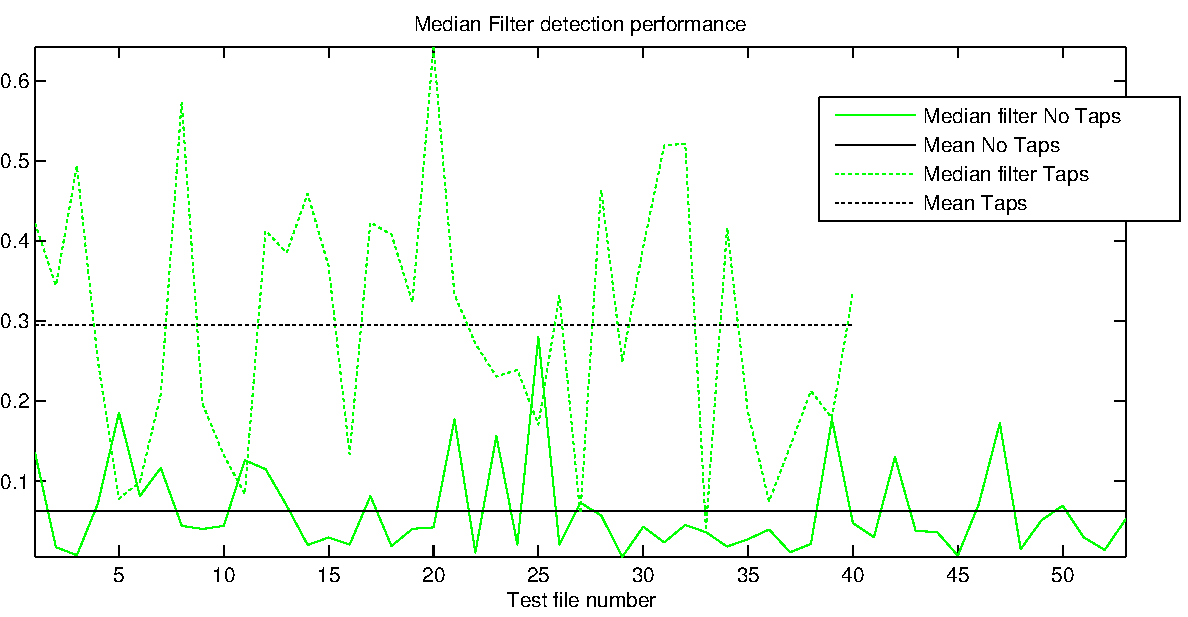
\includegraphics[width=12cm]{DetectPerfMedian.pdf}
  \begin{picture}(0,0)
%\put(-310,275){a)}
%\put(-310,135){b)}
\end{picture}}
\end{minipage}
\caption{Maximum detector response for files with either a tap or some speech.}
\label{fig:DetectPerfMedian.pdf}
\end{figure}

\subsubsection{False detection rate}

To evaluate the performance of any given detection algorithm the rate of false detections is often considered. Assuming that all positive detections were detected correctly, the false detection rate gives a measure of an algorithms sensitivity and therefore its performance.

In this comparison we will be comparing the Wavelet based detection algorithm, discussed in section~\ref{sec:WPdetection}, the STFT based UKD algorithm\cite{Subramanya2007} and a basic median based detection algorithm. Since all these detection algorithms investigated depend on various thresholds, it is important to construct a method for calibrating all methods so a valid comparison can be drawn. For this a set of 40 keyboard taps collected from a variety of sources was used. The threshold was set as the minimum value of the maximum responses of each tap for every model. In other words, the threshold was adjusted so that it would only just detect all 40 taps.

Figure~\ref{fig:maxes.pdf} shows the various maximum responses of each tap for all three detection methods. Had any of these methods produced a significantly lower response for only a few of the taps the calibration scheme chosen here would have put that detection method at a disadvantage. In this instance none of the methods produce significantly outlying responses. It is although noted that the Wavelet based detector does produce extremely high responses in some instances.

\begin{figure} %maxes.pdf
\centering
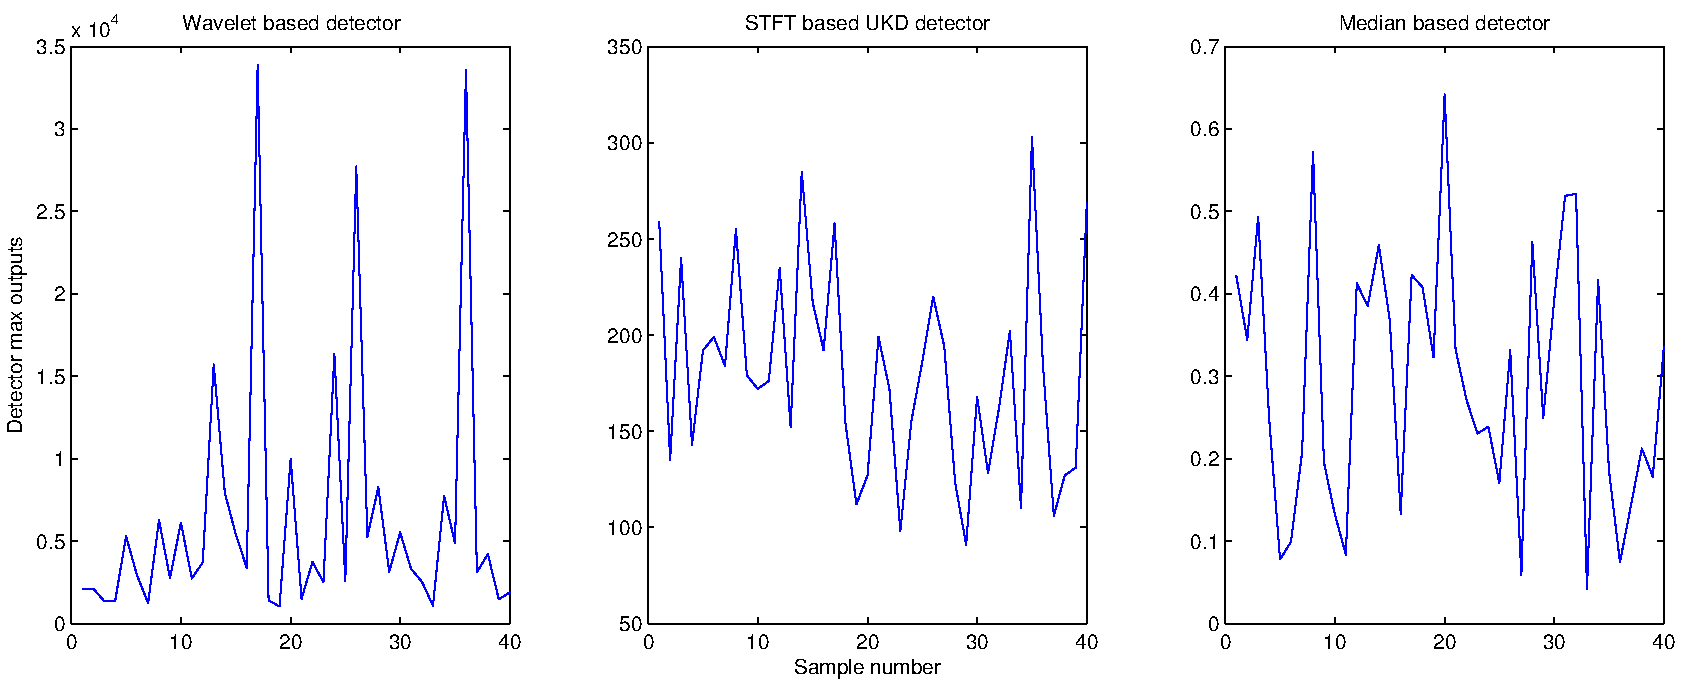
\includegraphics[width=120mm]{maxes.pdf}
\caption{Various detection algorithm response performance for the same 40 keystroke taps.}
\label{fig:maxes.pdf}
\end{figure}

Given the threshold set as described above, an additional 55 short audio segments (combined playing time of about 1 min) containing speech were analysed.

It was found that both the Wavelet and STFT based methods had 2 false detections while the median detector had 28 false detections. While the STFT UKD method might have identical performance to the Wavelet based method it should be noted that the UKD method requires a longer look-ahead and provides a coarser temporal resolution than the Wavelet based method.

\section{Discussion}\label{sec:WPdiscussion}
\subsection{Separation algorithm}

By visual inspection of Figures~\ref{fig:Separation_Residual_Example} through \ref{fig:SeparationWaveformExBig640.pdf} it is clear that the separation algorithm provides a reduction of speech while leaving transient noise events largely the same in the residual component. Audibly this effect is also clearly verified. Despite a distinct audible effect on the speech the tonal component alone manages a decreased maximum MSE from 5.2 to 3.2 as well as increasing the PSNR from 80.5 dB to 82 dB. While the maximum MSE is nearly halved in the tonal component of the signal, the original corruption site is still clearly visible in Figure~\ref{fig:SeparationError.pdf}. The original corruption is nearly inaudible in the tonal component and Figure~\ref{fig:SeparationErrorData.pdf} shows in more detail the waveform of the corruption site. The MSE might still be significant in Figure~\ref{fig:SeparationError.pdf} but Figure~\ref{fig:SeparationErrorData.pdf} reveals that this might mainly be due to phase shifts around the corruption site with am inaudible effect.

\subsection{Detection algorithms}
Two different, but related, detection algorithms have been presented in this chapter; the noise burst model algorithm and the AR filtering algorithm. These two have been compared to two other approaches; the UKD algorithm\cite{Subramanya2007} and a median filter algorithm. While the median filter algorithm provides a benchmark for one of the simplest approaches previously used for similar applications, the UKD algorithm represents the best alternative in the literature.

%Discussion of NBDetectionResults and NBResultsTest
It is clear from Figure~\ref{fig:NBDetectionResults} and Table~\ref{table:NBResultsTest} that both the Noise Burst and the UKD algorithm outperform the standard median filter approach. Figure~\ref{fig:NBDetectionResults}(a) shows the UKD algorithm being slightly more sensitive than the Noise Burst model, while in Figure~\ref{fig:NBDetectionResults}(b) the UKD appears slightly less sensitive to embedded taps while finding more false detections than the Noise Burst model. It is although worth noting that the keyboard strokes generally missed are the ones for which the pulse amplitude appears to not exceed that of the speech segment. For all methods tested this does appear to be a difficult detection scenario especially at low (for audio in general) sample rates of 16kHz. At higher sample rates, where the speech would take up a lower proportion of the bandwidth, the algorithms should perform better assuming that the noise pulse's spectrum is being limited by the current sample rate. Table~\ref{table:NBResultsTest} shows the Noise Burst algorithm being more sensitive than UKD while all tested algorithms maintain a low false detection rate. The median detector's good performance in the last test is probably explained by the relatively loud transients in the audio compared to the speech.

Figure~\ref{fig:NBDetCompare} specifically shows one of the strengths of the noise burst algorithm in relation to the UKD algorithm. While both algorithms catch elements of both keyboard strokes the UKD algorithm misses the initial pulse of the second keyboard stroke. Additionally the noise burst algorithm gives a clear estimate of the extent of the corruption. The detection rate results from Table~\ref{table:NBResultsTest} also shows similar results although again slightly in favour of the noise burst model.

In general the results presented in section~\ref{sec:WPdetectionNBresults} indicate that the noise burst model outperforms both the UKD and the median filter method. A significant issue with the noise burst model is although that it requires a good estimate for the variance of noise pulses for the algorithm to perform well in various scenarios which will have to be updated requiring additional algorithmic complexity. The results presented in this chapter has attempted to assess the algorithms on a variety of data but the amount of tuning required for the noise burst model to perform well does make a simple and general implementation infeasible.

The AR filter method was considerably easier to implement, more generally applicable and computationally simpler. Figure~\ref{fig:ARFilterDetectionResults} shows the results from a similar test to that of Figure~\ref{fig:NBDetCompare} with the AR filter method generally being more sensitive. While the AR filter method does appear to trigger more false detections, closer inspection of the underlying data does suggest that some of these are in fact secondary pulses while others are other spurious acoustic noise pulses. The only clearly falsely detected pulse is the detection of the sharp speech onset in the second speech segment. The same speech segment that the noise burst model falsely detected, as seen in Figure~\ref{fig:NBDetCompare}. As with the noise burst model the AR filter method also misses a detection although a different one in this case.

While the visible real world detection results, Figures~\ref{fig:ARFilterDetectionResults} and \ref{fig:NBDetCompare}, are informative, the problem of assessing objectively what qualifies as a false detection can be difficult. The Figures~\ref{fig:DetectPerfARFilt.pdf} - \ref{fig:DetectPerfMedian.pdf} provide clear representation of the range of excitation values for a set of 40 audio files with keyboard strokes and 53 files including speech and no noise pulses. The general margin between these two ranges indicate the robustness of the algorithm. It is seen from these plots the AR filter method, Figure~\ref{fig:DetectPerfARFilt.pdf}, and the UKD algorithm, Figure~\ref{fig:DetectPerfUKD.pdf}, clearly outperforms the median filter approach, Figure~\ref{fig:DetectPerfMedian.pdf}, which shows a significant overlap of the two ranges. While the AR filter approach has maximum responses with higher variance the UKD algorithm has a more consistent response. The lower variance of the UKD response is probably due to a smoothing effect by the larger size of the Fourier transform windows used in this procedure, since both method respond to similar wide band noise characteristics in the pulses. The two methods also have responses on very different scales so a direct comparison can be difficult but based on the relationship between the minimum response for a positive detection and the maximum response for a false detection the AR filter method provides an increased margin and thereby robustness. Other practical concerns speak in favour of the AR filter method as well. The AR filter method also provides provides higher temporal resolution, via the Wavelet Transform, than the UKD algorithm in addition to not requiring the additional look-ahead. Better temporal resolution provides more accurate detection and therefore more accurate restoration. Less required look-ahead in the algorithm makes real time implementations more feasible and reduces in-built latency.

%Although the algorithms generally performed well on the data sampled at 16kHz in this section, which is common in wide band VoIP applications, it should be noted that for audio recorded at higher sample rates the
%narrowband telecommunication systems work against these detection algorithms by having a less sparse spectrum.
\section{Conclusions}\label{sec:WPconclusions}

This chapter has explored a variety of noise pulse detectors for the express purpose of detecting keyboard strokes for a real time communication system. The pulses created by the keyboard stroke was found to generally consist of a number of noise pulses each associated with various mechanical interactions with the keyboard itself. All of these pulses had varying amplitudes and timing in relation to each other depending on the a range of parameters. The individual detection of these different pulses appears to be the only feasible approach to the detection step due to this variability. Two detectors were developed and tested in this section; the noise burst model and the AR filter method. These were compared and contrasted with a state of the art algorithm for this purpose, the UKD algorithm\cite{Subramanya2007}, and a basic and largely legacy approach using a median filter.

Tests suggested that with careful tuning the noise burst model performed at least as well as the UKD algorithm on the data sets used, while providing additional functionality. It was although also noted that the algorithm was reliant on a variety of parameters that complicated the application of the algorithm and could limit the general applicability of the algorithm.

While it is difficult to conclusively state, based on the results in section~\ref{sec:WPresults}, that the AR filter method is superior to the noise burst model and the UKD algorithm, considering practical implementation concerns it provides a detection performance at least on par with the competition without the in-built latency and poor temporal resolution of the UKD algorithm or the required training and complexity of the noise burst model. Predictably, all algorithms tested outperformed the median filter algorithm.

\subsection{Possible future work}
Based on the same background assumption that led to the development of the multi-channel APR system in chapter~\ref{ch:MultichannelAPR}, it is possible to extend the detection process to multiple channels. While not necessarily providing the same information through ToF it is still possible to improve performance through additional correlated sources as clearly shown from the results in chapter~\ref{ch:MultichannelAPR} if with nothing more than simple majority voting (median/mode processing).

% ------------------------------------------------------------------------


%%% Local Variables:
%%% mode: latex
%%% TeX-master: "../thesis"
%%% End: \ 